\documentclass[12pt,a4paper,spanish]{article} 

\usepackage{graphicx} %option specific for pdfLatex compilation
\usepackage{makeidx}
\usepackage{lscape}

\usepackage[spanish]{babel}
\usepackage[utf8]{inputenc} 
\usepackage{indentfirst}

\usepackage[margin=1in]{geometry}


\begin{document}
\begin{titlepage}
\begin{center}

% Upper part of the page. The '~' is needed because \\
% only works if a paragraph has started.

\textsc{\LARGE \textbf{Universidad de Buenos Aires}}\\%[1cm]
\vfill
\textsc{\LARGE \textbf{Técnicas de Programación Concurrente I }}\\%[0.5cm]
\vfill
\textsc{\LARGE \textbf{(75.59)}}\\%[0.5cm]
\vfill
% Title
%\HRule \\[0.4cm]
\vfill
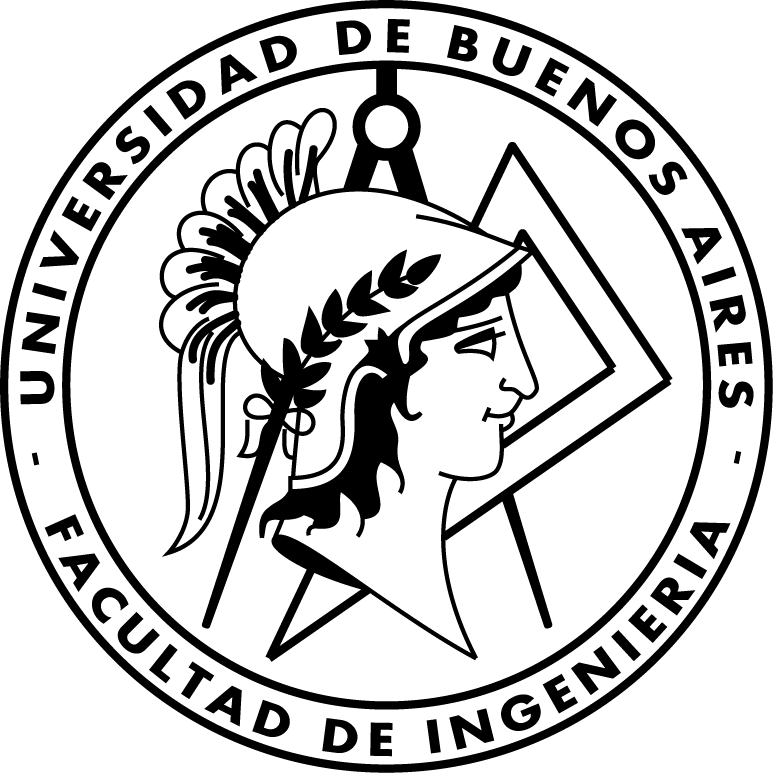
\includegraphics[scale=1.25]{./logo.png}~\\[2cm]
%\HRule \\[1.5cm]
{ \huge \bfseries Trabajo Práctico Nº 1}\\%[0.25cm]
\vfill
%{ \huge \bfseries Grupo 8}\\%[0.25cm]
%\vfill
{\Large
\begin{tabular}{|c|c|c|}
\hline
Nombre y apellido & Padrón & Mail \\
\hline
Florencia Bosch & 91867 & florb\_128@hotmail.com \\
\hline
Javier Choque & 92079 & javierchoque21@gmail.com \\
\hline
Pablo Musumeci & 92165 & pablomusumeci@yahoo.com.ar\\
\hline
\end{tabular}
}
\vfill

% Bottom of the page
{\large \today}

\end{center}
\end{titlepage}

\newpage
\tableofcontents
\newpage
\section{Diseño}

\section{Hipótesis}

\begin{itemize}
	\item Consideramos que cuando un auto es enviado a la salida por el Jefe de Estación,
	el mismo sale del sistema de manera instantánea, sin tener que hacer una cola
	para salir de la estación.

	\item El administrador no tiene prioridad sobre los empleados al momento de consultar
	el saldo en la caja, y debido a esto, cuando desea hacerlo debe aguardar su turno para
	trabajar de manera exclusiva con la caja, al igual que cualquier empleado.
\end{itemize}

\subsection{Casos de uso}

\begin{itemize}
	\item Inicar simulación: El actor que dispara este caso de uso es el usuario
	que desea iniciar la simulación. Para iniciar el programa se debe ejecutar el
	proceso \texttt{procesoPrincipal}, el cual se encarga de
	lanzar a los otros procesos involucrados en el funcionamiento de la simulación.

	Es necesario que la ejecución del proceso principal se realize con los parámetros
	que indican la cantidad de empleados (por medio de la expresión \texttt{-e} o \texttt{--empleados})
	y la cantidad de surtidores (\texttt{-s} o \texttt{--surtidores})que que tendrá la
	estación de servicio.

	Ejemplo:

	\texttt{./procesoPrincipal -e 5 -s 7}
\end{itemize}

\section{Procesos del proyecto}

	\subsection{Generador de Autos}
		
		Este proceso es el encargado de crear los autos que llegan a la estación. Para
		dicho propósito, genera un auto en intervalos de tiempo elegidos de forma aleatoria. 
		Cada auto está representado por un ID y una cantidad de dinero que va a gastar en la estación.

		El Generador de Autos interactúa con el Jefe de Estación, y dicha interacción se puede
		asemejar al problema \textbf{Producer - Consumer}, debido a que el Generador produce
		los autos que el Jefe de Estación va a recibir. 

		Al analizar este problema, debemos tener en cuenta que el \textbf{producer} no debería
		agregar información al medio que comparte con el consumer, si el mismo se encuentra lleno.
		En esta situación optamos por enviar a dormir al proceso generador, por un tiempo
		aleatorio, y volver a intentar escribir en el buffer cuando se despierte.

	\subsection{Jefe de Estación}
		Este proceso se encarga de recibir los autos nuevos que van llegando a la estación. 
		En este caso, el Jefe de Estación es el \textbf{consumer} de información, y debe
		cerciorarse de no intentar extraer información del buffer si el mismo esta vacío.

		Una vez que logró extraer un automóvil del buffer exitosamente, debe asignarle 
		un empleado al auto recibido, en caso de que exista algun empleado disponible 
		en ese mismo instante, caso contrario,deberá redirigir el mismo hacia la salida.
		
		Para esto, el proceso explora un array de valores lógicos (booleanos), que representan la disponibilidad de los empleados. La posición del booleano en el array es tambien el ID de empleado (no confundir con el PID del proceso empleado). Una vez hallado al empleado, se marca el valor lógico correspondiente como ``Ocupado''. Luego se graban los datos del auto en un pipe compartido con le proceso Empleado.

	\subsection{Empleado}
	
	Este proceso representa el accionar de un empleado cuando atiende un auto. El proceso espera un auto por un pipe, cuando lo lee, busca un surtidor libre, lo cual se representa por medio de un semáforo que se encarga de llevar la cuenta de cuantos surtidores disponibles hay. Una vez tomado el surtidor, procede a atender el auto. En nuestra simulación, atender un auto se traduce en introducir una demora (sleep) antes de grabar el monto cobrado en la caja. Dicha demora se determinará por medio de una cuenta realizada con la cantidad de dinero que el auto tiene (el cual es determinado de manera aleatoria al momento de su creación). 

	Vale aclarar que el sleep mencionado recién es utilizado simplemente para simular la utilización del surtidor, cuya implementación escapa del ámbito de este proyecto, y no es utilizado como mecanismo de coordinación entre ningún par de procesos.
	
	Una vez que termina el tiempo de atención del auto, el empleado busca el control de la caja para grabar lo recaudado. Esta operación es un problema de concurrencia entre todos los procesos empleados, y debe ser coordinada mediante un semáforo binario (es decir, el semáforo está tomado o no).
	
	\subsection{Administrador}
	
	El proceso administrador tiene la facultad de consultar el valor guardado en la caja. Puede hacerlo en cualquier momento, y su consulta sobre la caja esta controlada de la misma forma que el empleado. La diferencia con el empleado es que el Administrador no espera a un auto, sino que puede consultar en cualquier momento.
	
	\section{Diagrama esquemático de interacciones}
	
	Ver figura \ref{diagrama}

\begin{figure}
\label{diagrama}
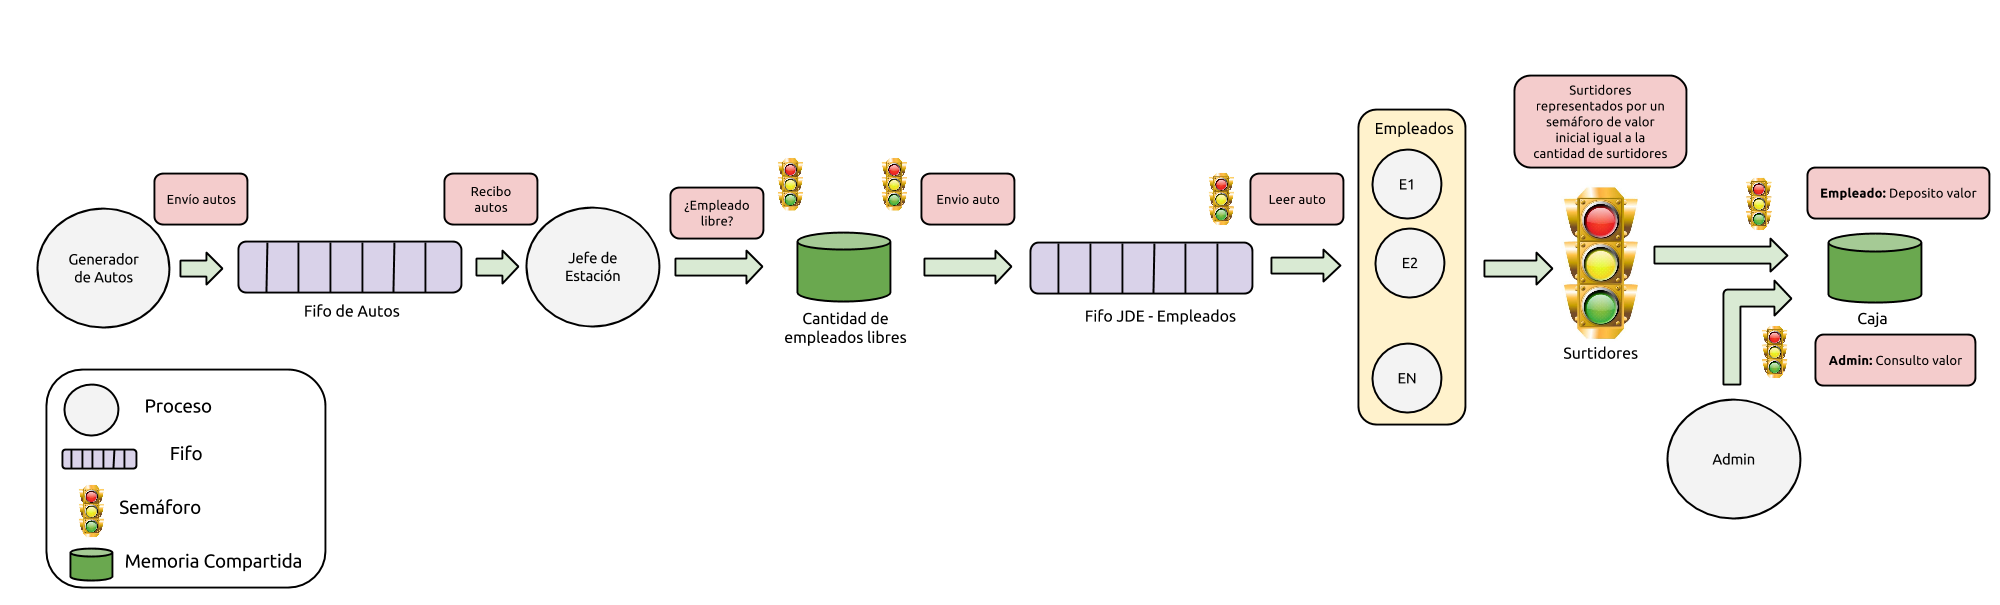
\includegraphics[width=1.0\textwidth]{esquema.png}
\caption{Diagrama esquemático de interacciones}
\end{figure}

	\section{Datos compartidos entre procesos}
	
	\begin{itemize}
	
	\item Generador de Autos - Jefe de Estación:
		\begin{itemize}
			\item Fifo \texttt{files/generador.jde} para envío de los autos
		\end{itemize}
	
	\item Jefe de Estación - Empleado:
	\begin{itemize}
		\item Fifo \texttt{files/jde.empleado} para envío de los autos
		\item Memoria compartida (arreglo) para detectar empleado disponible
		% \item Mecanismo para tener bloqueado al empleado cuando esta idle
	\end{itemize}
	
\item Empleado - Empleado (surtidores):
	\begin{itemize}
		\item Semáforo \texttt{files/semaforo.surtidores} que representa la 
		cantidad de surtidores libres, y controla el acceso a los mismos.
	\end{itemize}

	\item Empleado - Empleado (caja):
	\begin{itemize}
		\item Memoria compartida que representa la caja
		\item Semáforo \texttt{} para acceder a la caja
	\end{itemize}

	\item Empleado - Administrador:
	\begin{itemize}
		\item Memoria compartida que representa la caja
		\item Semáforo \texttt{} para acceder a la caja
	\end{itemize}

	\end{itemize}

	\section{Diagrama de estados del proceso Jefe De Estación}

	\begin{figure}
	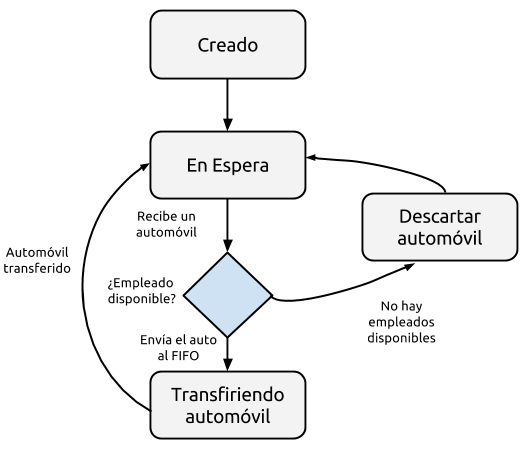
\includegraphics[width=1.0\textwidth]{FSM_JDE.png}[h]
	% https://docs.google.com/drawings/d/1fSqCpKnnYxksGUfpufRSJbsfxkYRRuSEGUDkyJf5Sf0/edit?usp=sharing
	\caption{FSM del Jefe de Estación}
	\end{figure}



\end{document}
